\documentclass{article}
\usepackage{graphicx, alphabeta, hyperref, xcolor, amsmath, float} % Required for inserting images

\title{Αριθμητική Ανάλυση - 2η Εργασία}
\author{Αλέξανδρος Καραμουχτάρης | 4369}
\date{January 2024}

\begin{document}

\maketitle

\setcounter{section}{4}
\section*{Εισαγωγή}
\begin{center}
Ο κώδικας για τη συγκεκριμένη εργασία έχει γραφεί στη γλώσσα Python κι έχει γίνει χρήση των πακετών "numpy" και "matplotlib". Είναι κατάλληλα σχολιασμένος και κάθε συνάρτηση περιλαμβάνει το δικό της docstring, το οποίο εξηγεί αναλυτικά τη λειτουργικότητά της, τις παραμέτρους που δέχεται και το τι επιστρέφει. Τα σχόλια του παραπάνου είδους έχουν ενισχυθεί από το Chat-GPT ώστε να είναι πιο σαφή και κατανοητά. Για καθεμιά από τις ασκήσεις, υπάρχει ο δικός της φάκελος, ο οποίος περιλαμβάνει τις συναρτήσεις που χρησιμοποιούνται σε ένα αρχείο "functions.py" και τον κορμό του προγράμματος σε ένα άλλο αρχείο "main.py". Επιπλέον, υπάρχει το αρχείο "global\_functions.py" το οποίο βρίσκεται στο "parent directory" και είναι διαθέσιμο να χρησιμοποιηθεί σε κάθε άσκηση. Τέλος, χρησιμοποιήθηκε Git και Github και το repository της εργασίας ειναι διαθέσιμο \href{https://github.com/AlexandrosKaram/Numerical-Analysis-2.git}{\color{blue}{εδώ}}.
\end{center}

\section{Πέμπτη Άσκηση}
Στην πρώτη άσκηση μας ζητείται να προσεγγίσουμε τη συνάρτηση του ημιτόνου στο διάστημα \([-π, π]\). Καθεμία από τις συναρτήσεις που υλοποιήθηκαν, δέχεται ως ορισμάτα:

\begin{itemize}
  \item 10 σημεία που λειτουργούν ως δείγμα.
  \item 200 τιμές του \( x \) εντός του διαστήματος για τις οποίες επιστρέφεται σε μια λίστα η \( y \)-προσέγγιση τους.
\end{itemize}

Για κάθε φορά που εκτελέιται ο αλγόριθμος, τα αποτελέσματα θα είναι διαφορετικά, καθώς το δείγμα υπολογίζεται με τυχαίο και ανομοιόμορφο τρόπο. Τα αποτελέσματα που θα σχολιαστούν παρακάτω θα είναι με βάση τις τιμές του \( x \):

\[
\{-3.14159, -2.15252, -1.69569, -0.71119, -0.23925, 0.30665, 0.57424, 0.99677, 2.20463, 3.14159\}.
\]

Τα διαγράμματα σφάλματος εμφανίζονται με τη συνάρτηση \texttt{display\_error\_graph()} η οποία εντοπίζεται στο αρχείο \texttt{"graph\_error.py"}.

\subsection{Πολυωνυμική Προσέγγιση}
Για την πολυωνυμική προσέγγιση του ημιτόνου θα υλοποιηθεί η συνάρτηση \texttt{Lagrange()} η οποία βασίζεται στον τύπο 
\[
p_n(x) = \sum_{i=0}^{n} y_i \cdot L_i(x),
\]
όπου 
\[
L_i(x) = \frac{(x - x_0) \cdots (x - x_{i-1})(x - x_{i+1}) \cdots (x - x_n)}{(x_i - x_0) \cdots (x_i - x_{i-1})(x_i - x_{i+1}) \cdots (x_i - x_n)},
\]
για \( i = 0, \ldots, n \).\\\\
Από το παρακάτω διάγραμμα,
\begin{center}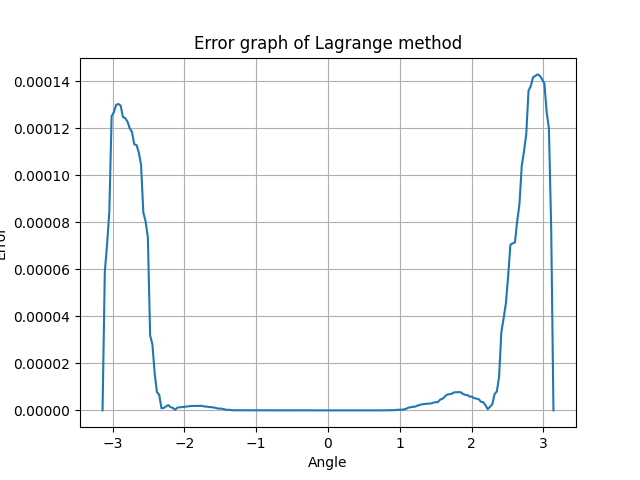
\includegraphics[width=\linewidth]{lagrange.png}\end{center}
είναι εμφανές ότι η μέθοδος Lagrange είναι αρκετά αποτελεσματική στην προσέγγισή της, καθώς υπολογίζει το ημίτονο με μέσο σφάλμα 2.40126e-05, δηλαδή 0.0000240126. Η ακρίβεια είναι κατα μέσο όρο στα 4 δεκαδικά ψηφία. Παρατηρούμε ότι το μεγαλύτερο σφάλμα παρουσιάζεται κοντά στα άκρα του διαστήματος. Αύτο συμβαίνει λόγω της χαμηλής πυκνότητας του δείγματος σε εκείνα τα σημεία. Για παράδειγμα, μετά το -3.14159 η επόμενη τιμή του \( x\) είναι -2.15252, περίπου μία μονάδα μακριά, καθυστώντας δύσκολη την προσέγγιση του ημιτόνου σε εκείνο το διάστημα.

\subsection{Splines}
Θα προσεγγίσουμε το ημίτονο με τη μέθοδο της φυσικής κυβικής σφήνας χρησιμοποιώντας τον παρακάτω τύπο
\[
S_i(x) = a_i(x) + b_i(x - x_i) + c_i(x - x_i)^2 + d_i(x - x_i)^3
\]
για \(i = 1, \cdots , n-1\)\\\\
Οι παράμετροι μας θα υπολογιστούν ως εξής:
\begin{enumerate}
    \item Θα υπολογιστούν δύο βοηθητικές παράμετροι
    \[
    δ_i = x_{i+1} - x_i
    \]
    \[
    Δ_i = y_{i+1} - y_i
    \]
    για \( i = 1, \ldots, n-1 \).\\
    \item Θα επιλυθεί το γραμμικό σύστημα \(Ac = b\) όπου
    \[
    A = \begin{bmatrix}
    1 & 0 & 0 \\
    δ_1 & 2δ_1 + 2δ_2 & δ_2 & \ddots \\
    0 & δ_2 & 2δ_2 + 2δ_3 & δ3 \\
      & \ddots & \ddots & \ddots & \ddots & \\
      & & & δ_{n-2} & 2δ_{n-2} + 2δ_{n-1} & δ_{n-1} \\
      & & & 0 & 0 & 1\
      
    \end{bmatrix}
    \]
    \[
    b = \begin{bmatrix}
        0 \\
        3(\frac{Δ_2}{δ_2} - \frac{Δ_1}{δ_1}) \\
        \\
        \vdots \\
        \\
        3(\frac{Δ_{n-1}}{δ_{n-1}} - \frac{Δ_{n-2}}{δ_{n-1}}) \\
        0 \        
    \end{bmatrix}
    \]
    Η λύση του συστήματος υπολογίζεται με συνάρτηση αποσύνθεσης \texttt{PA = LU} η οποία είχε υλοποιηθεί στην πρώτη υποχρεωτική εργασία. Ο κώδικας για τη συγκεκριμένη συνάρτηση - \texttt{solve\_linear\_system()} βρίσκεται στο αρχείο \texttt{"helper.py"}. Το αποτέλεσμα θα είναι κι οι τιμές που θα δέχεται η παράμετρός μας \texttt{c}.
    \item Τώρα μπορούν να υπολογιστούν κι οι υπόλοιπες μας παράμετροι
    \[
    a_i = y_i
    \]
    \[
    d_i = \frac{c_{i+1} - c_i}{3δ_i}
    \]
    \[
    b_i = \frac{Δ_i}{δ_i} - \frac{δ_i}{3} (2c_i + c_{i+1})
    \]
    για \( i = 1, \ldots, n-1 \).\\
\end{enumerate}
Αφού έχουμε πλέον όλα τα απαραίτητα στοιχεία, θα δούμε για το καθένα από τα 200 \(x\) σε ποιο υποδιάστημα του [-π, π] βρίσκεται και θα υπολογίσουμε με τη βοήθεια του τύπου μας τις καινούργιες τιμές \(y\).\\\\
Στο διάγραμμα:
\begin{center}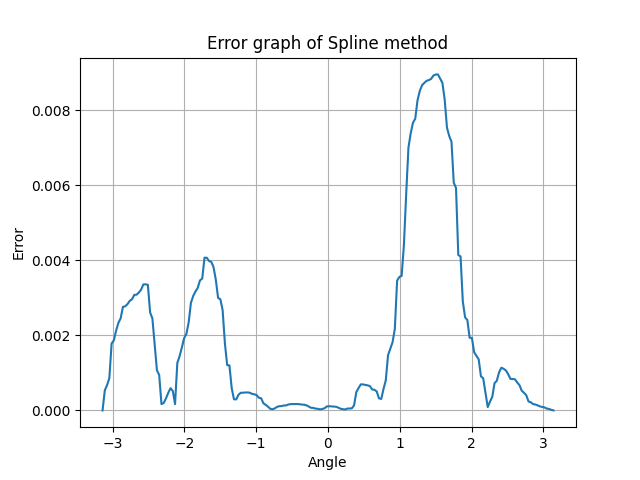
\includegraphics[width=\linewidth]{splines.png}\end{center}
παρατηρούμε ότι η ακρίβεια στη μέση του διαστήματος είναι πολύ ικανοποιητική. Εκεί που αραιώνει όμως το δείγμα μας εξουθενώνεται κι η ακρίβεια. Σε γενικές γραμμές η επιτυχία κυμαίνεται στα 2 με 3 δεκαδικά ψηφία και το μέσο σφάλμα είναι 0.0019518331. Συνεπώς, η προσέγγιση αυτή αποδεικνύεται με το συγκεκριμένο δείγμα λιγότερο αποτελεσματική από την πολυωνυμική.

\subsection{Ελάχιστα Τετράγωνα}
Η τρίτη κι η τελευταία μας μέθοδος είναι αυτή των ελάχιστων τετραγώνων. Για τη συγκεκριμένη άσκηση θα χρησιμοποιηθεί η γραμμική προσέγγιση, δηλαδή η εξίσωση θα είναι πρώτου βαθμού και θα συμμορφώνεται με τον τύπο
\[
y_i = mx_i + b
\]
Οι συντελεστές m και b υπολογίζονται ως εξής:\\
\[
m = \frac{n\sum(xy) - \sum x \sum y}{n\sum(x^2) - (\sum x)^2}
\]
\[
b = \frac{\sum y - m\sum x}{n}
\]
Το κάθε άθροισμα $\sum$ υπολογίζεται για \( i = 1, \ldots, n \).\\\\
Το παρακάτω διάγραμμα σφάλματος
\begin{center}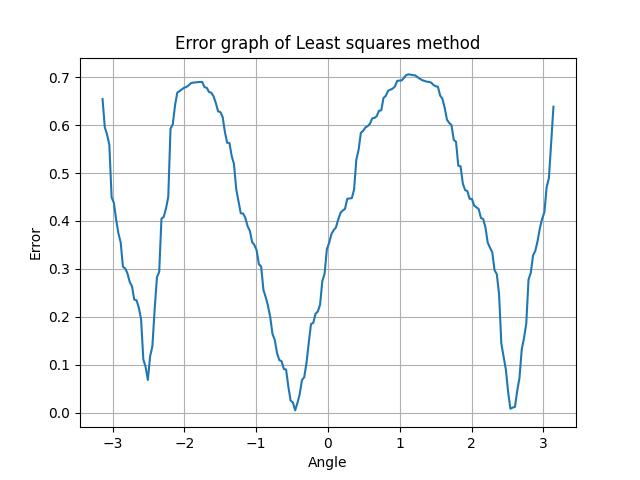
\includegraphics[width=\linewidth]{ls.png}\end{center}
εύκολα μας οδηγεί στο συμπέρασμα ότι αυτή η μέθοδος δεν είναι καθόλου αποτελεσματική καθώς αδυνατεί να υπολογίσει με ικανοποιητική ακρίβεια τις περισσότερες τιμές, πέφτοντας κατά μέσο όρο 0.4255062769 έξω από το αποτέλεσμα (0 - 1 δεκαδικό ψηφίο ακρίβεια).

\section{Έκτη Άσκηση}
Στη συγκεκριμένη άσκηση θα υπολογιστεί μία προσέγγιση του ολοκληρώματος του ημιτόνου στο διάστημα $[0, \frac{π}{2}]$ με τις παρακάτω μεθόδους.

\subsection{Κανόνας Τραπεζίου}
Η συνάρτηση \texttt{trapezoidal\_integration()}:
\begin{enumerate}
    \item Δέχεται ως όρισμα το διάστημα στο οποίο θα υπολογίσει το ολοκλήρωμα του ημιτόνου
    \item Χωρίζει το διάστημα μας σε 10 ισομήκη υποδιαστήματα, δηλαδή υπολογίζει 11 τιμές \(x\) όπου $\{x_0=a, x_1, ..., x_{10}=b\}$ με a, b τα άκρα του αρχικού διαστήματος και
    \[
    x_i = x_0 + k\frac{b - a}{n}
    \]
    k = 0, ..., 10
    \item Υπολογίζει το ημίτονο για αυτά τα x.
    \item Επιστρέφει το τελικό αποτέλεσμα το οποίο δίνεται από τον τύπο 
\[
\int_{a}^{b} f(x) \, dx \approx \frac{b - a}{2n} \left( y_0 + y_n + 2 \sum_{k=1}^{n-1} y_k \right)
\]
\end{enumerate}
Για να υπολογίσουμε το θεωρητικό σφάλμα θα χρειαστούμε τη δεύτερη παράγωγο του ημιτόνου, δηλαδή 
\[
f"(x) = -sin(x)
\]
Το σφάλμα \(e\) υπολογίζεται από τον τύπο:
\[
|e| \leq \frac{(b - a)^3}{
12n^2} M
\]
όπου \(M\) η μέγιστη κατά απόλυτη τιμής της $f"(x)$ στο διάστημα $[0, \frac{π}{2}]$, δηλαδή 1.
Επομένως η σχέση μας απλοποιείται ως:
\[
|e| \leq \frac{π^3}{9600} = 0.00322982048
\]
Το πραγματικό σφάλμα βλέπουμε από την κονσόλα ότι είναι 0.0020570136456428134 (αρκετά κοντά με το θεωρητικό).

\subsection{Simpson}
Η προσέγγιση με τη μέθοδο του Simpson είναι αρκετά παρόμοια με εκεινή του τραπεζίου με τη διαφορά οτι ο τύπος μας είναι αυτός:
\[
\int_{a}^{b} f(x) \, dx \approx \frac{b - a}{3n} \left[ f(x_0) + 4 \sum_{k=1}^{n/2} f(x_{2k-1}) + 2 \sum_{k=1}^{n/2-1} f(x_{2k}) + f(x_n) \right]
\]
Δηλαδή τα \(x\) δεν ενώνονται με ευθύγραμμα τμήματα, αλλά με παραβολές.\\\\
Για τη μέθοδο Simpson, το θεωρητικό σφάλμα \(e\) υπολογίζεται από τον τύπο
\[
|e| \leq \frac{(b-a)^5}{180n^4}M
\]
όπου M η μέγιστη τιμή της τέταρτης παραγώγου της $f(x) = sin(x)$, που στη συγκεκριμένη περίπτωση είναι ίση με 1.\\
Έτσι, το αποτέλεσμα μας απλοποιείται ώς:
\[
|e| \leq \frac{π^5}{57600000} = 0.00000531284
\]
Το πραγματικό σφάλμα για το πρόγραμμα μας στη γλώσσα Python είναι 3.3922209004000337e-06 δηλαδή περίπου 0.0000033922209 (επίσης αρκετά κοντά με το θεωρητικό).

\subsection{Σύγκριση}
Τα θεωρητικά σφάλματα είναι αρκετά κοντά με τα πραγματικά. Επιπλέον, και στις δύο περιπτώσεις αποδεικνύεται ότι η μέθοδος του Simpson έχει μεγαλύτερη ακρίβεια από την τραπεζοϊδή.
\begin{table}[h!]
\centering
\begin{tabular}{|l|c|c|}
\hline
\textbf{Method} & \textbf{Theoretical Error} & \textbf{Actual Error} \\
\hline
Trapezoidal Method & \( 0.00322982048 \) & \( 0.002057013645 \) \\
\hline
Simpson's Method & \( 0.00000531284 \) & \( 0.0000033922209 \) \\
\hline
\end{tabular}
\end{table}

\section{Έβδομη Άσκηση}
Στην παρούσα άσκηση εξετάζεται η δυνατότητα πρόβλεψης των τιμών κλεισίματος των μετοχών χρησιμοποιώντας τη μέθοδο των ελάχιστων τετραγώνων για την προσαρμογή πολυωνυμικών συναρτήσεων διαφόρων βαθμών στα δεδομένα τιμών.\\\\
Στο αρχείο \texttt{functions.py} υλοποιούνται οι τρεις συναρτήσεις που θα χρειαστούμε. Για την επίλυση των απαραίτητων γραμμικών συστημάτων χρησιμοποιείται η συνάρτηση \texttt{linalg.solve()} της βιβλιοθήκης \texttt{numpy}. Σε προηγούμενη άσκηση χρησιμοποιήθηκε συνάρτηση που υλοποίησα προσωπικά, όμως για λόγους ευκολίας και προσαρμογής με τις υπόλοιπες λειτουργίες της \texttt{numpy} τώρα χρησιμοποιείται η έτοιμη συνάρτηση.\\\\
Για δεδομένα χρησιμοποιήθηκαν τα 10 κλεισίματα για τις εταιρίες \texttt{ΟΠΑΠ} και \texttt{ΔΕΗ} της χρονικής περιόδου 9-22/6/2023 (Γενέθλια 23/6). Στη συνέχεια πραγματοποιήθηκαν προβλέψεις με τις συναρτήσεις μας για την επόμενη και άλλες πέντε ημέρες. Τα αποτελέσματα είναι τα εξής:
\begin{table}[ht]
\begin{tabular}{|l|l|l|}
\hline
\multicolumn{3}{|c|}{\textbf{ΟΠΑΠ}} \\
\hline
\textbf{Μέθοδος} & \textbf{Επόμενη μέρα} & \textbf{Μέρες 2-6} \\
\hline
Δευτέρου Βαθμού & 15.77 & 15.48, 15.13, 14.74, 14.29, 13.79 \\
\hline
Τρίτου Βαθμού & 15.88 & 15.85, 15.90, 16.07, 16.39, 16.87 \\
\hline
Τετάρτου Βαθμού & 15.95 & 16.41, 17.48, 19.43, 22.56, 27.21 \\
\hline
\end{tabular}
\label{table:opap_stock_closings}
\end{table}

\begin{center}
\begin{table}[H]
\begin{tabular}{|l|l|l|}
\hline
\multicolumn{3}{|c|}{\textbf{ΔΕΗ}} \\
\hline
\textbf{Μέθοδος} & \textbf{Επόμενη μέρα} & \textbf{Μέρες 2-6} \\
\hline
Δευτέρου Βαθμού & 10.01 & 9.96, 9.90, 9.83, 9.76, 9.68 \\
\hline
Τρίτου Βαθμού & 10.01 & 9.97, 9.92, 9.87, 9.82, 9.76 \\
\hline
Τετάρτου Βαθμού & 9.98 & 9.74, 9.26, 8.47, 7.25, 5.47 \\
\hline
\end{tabular}
\label{table:deh_stock_closings}
\end{table}    
\end{center}\
Παρατηρούμε ότι ενώ για την επόμενη μέρα οι προβλέψεις των μεθόδων μας είναι εν μέρη ρεαλιστικές, στις επόμενες τα αποτελέσματα αδυνατούν να συμβιβαστούν με την πραγματικότητα. Μάλιστα, όσο ανεβαίνει ο βαθμός της μεθόδου, τόσο πιο πολύ ξεφεύγουν τα αποτελέσματα (overfitting) καθώς είναι σχεδιασμένες για να προσεγγίζουν τιμές πιο σύνθετων καμπυλών.\\
Τέλος, μπορούμε να συμπεράνουμε ότι οποιαδήποτε έκδοση της μεθόδου των ελάχιστων τετραγώνων δεν είναι κατάλληλη για να προβλέψει την πορεία μετοχών στο χρηματιστήριο, καθώς υπάρχουν πολλοί εξωτερικοί παράγοντες που την επηρεάζουν, τους οποίους μια μαθηματική μέθοδος δεν μπορεί να λάβει υπ' όψην.

\end{document}
